% ------------------------------------------------------------------
%  Supplementary Information for the LongPhase 2 manuscript
%  Build:  latexmk -pdf Supplementary.tex
% ------------------------------------------------------------------
\documentclass[11pt,a4paper]{article}
\usepackage[utf8]{inputenc}
\usepackage[T1]{fontenc}
\usepackage{lmodern}
\usepackage[margin=2.2cm]{geometry}
\usepackage{graphicx}
\usepackage{booktabs}
\usepackage{longtable}
\usepackage{array}
\usepackage{amsmath}
\usepackage{xspace}
\usepackage{xcolor}
\usepackage{caption}
\usepackage[super,sort&compress,numbers]{natbib}
\usepackage[hidelinks]{hyperref}
\usepackage{url}

\graphicspath{{figures/}{figures/supp/}}
\bibliographystyle{naturemag}
\setcitestyle{super,open={},close={}}
\captionsetup{labelfont=bf,font=small,justification=raggedright,singlelinecheck=false}

\newcommand{\toolname}{LongPhase~2\xspace}
\newcommand{\longphase}{LongPhase\xspace}
\newcommand{\whatshap}{WhatsHap\xspace}
\newcommand{\hapcut}{HapCUT2\xspace}
\newcommand{\todo}[1]{\textcolor{red}{[#1]}}
\newcommand{\code}[1]{\texttt{\small #1}}

% supplementary numbering
\renewcommand{\figurename}{Supplementary Fig.}
\renewcommand{\tablename}{Supplementary Table}
\newcolumntype{L}[1]{>{\raggedright\arraybackslash}p{#1}}

\title{Supplementary Information\\[6pt]
\large \toolname: uncertainty-aware co-phasing of small variants, structural variants and DNA methylation from long reads}
\author{Jyun-Hong Lin, \todo{co-authors}, Yao-Ting Huang}
\date{}

\begin{document}
\maketitle

\tableofcontents
\clearpage

% ==================================================================
\section*{Supplementary Notes}
\addcontentsline{toc}{section}{Supplementary Notes}

\subsection*{Supplementary Note 1. Reading the phasing graph export}
With \code{--dot}, \code{longphase phase} writes one file per chromosome, \code{<prefix>.<chrom>.dot}, containing one line per voting pair, \code{P.a -> Q.b [label=w]}, where \code{P} and \code{Q} are 1-based positions, \code{a}, \code{b} $\in \{1, 2\}$ index the reference (1) and alternate (2) allele, and \code{w} is the weighted haplotype vote accumulated at \code{P} for that allele at the time the vote was cast. The companion VCF carries, for every phased variant, the fields \code{INFO/H1}, \code{INFO/H2} (weighted votes for haplotype 1 and 2) and \code{INFO/PE} (their normalized Shannon entropy). The \code{gnn} sub-command reads both files; users who wish to inspect why a variant was unphased can therefore reconstruct its local window without re-running the phaser.

\subsection*{Supplementary Note 2. Reproducing the demonstration}
The repository ships a 500-kb demonstration (chr1:121.5--122.0~Mb; \code{demo/demo.sh}) that runs \code{modcall}, SNV-only and four-class \code{phase}, \code{gnn} correction of both outputs and \code{compare} against a truth VCF, and prints switch errors, phased SNV counts and Hamming distance for the four configurations. Total runtime is under two minutes on four threads.

\clearpage
% ==================================================================
\section*{Supplementary Tables}
\addcontentsline{toc}{section}{Supplementary Tables}

\begin{table}[h]
\caption{\textbf{Node features of the graph neural network.} Each allele node of a window carries 31 features; \# is the 1-based index in the feature vector (\code{GNNProcess.cpp}, \code{f[0]}--\code{f[30]}), listed here by group rather than by index. $h_1$, $h_2$: weighted haplotype votes (taken from the DOT edge labels when available, otherwise from \code{INFO/H1}, \code{INFO/H2}); PE: phasing entropy; PS: phase set; ``centre'' is the trigger variant of the window. Genomic-context features are computed from the reference when \code{-r} is given and are zero otherwise.}
\label{tab:nodefeat}
\small
\begin{tabular}{@{}r L{3.3cm} L{9.6cm}@{}}
\toprule
\# & Feature & Definition \\
\midrule
\multicolumn{3}{@{}l}{\textit{Phasing evidence (16)}}\\
1 & PE & normalized Shannon entropy of $(h_1, h_2)$, 0--1 bit \\
2 & HP & haplotype of this allele node (genotype index) \\
3 & gt\_ref & genotype index of the reference allele (0) \\
4 & gt\_alt & genotype index of the alternate allele (1) \\
5 & is\_center & 1 if the variant is the window trigger \\
6 & is\_same\_ps & 1 if the variant shares the trigger's PS \\
7 & allele & 0 for the reference-allele node, 1 for the alternate-allele node \\
8 & rel\_offset & (pos $-$ pos$_c$) / max$|$pos $-$ pos$_c|$ over the window, signed \\
9 & H1 & $h_1$ \\
10 & H2 & $h_2$ \\
11 & total\_votes & $h_1 + h_2$ \\
12 & vote\_ratio & $\max(h_1,h_2)/(h_1+h_2)$ \\
13 & log\_total & $\log_2(1 + h_1 + h_2)$ \\
14 & log\_h1 & $\ln(1 + h_1)$ \\
15 & log\_h2 & $\ln(1 + h_2)$ \\
25 & rel\_vote\_depth & $\log_2\big((h_1+h_2)/\overline{(h_1+h_2)}_{\pm 10\,\mathrm{variants}}\big)$ \\
\addlinespace
\multicolumn{3}{@{}l}{\textit{Genomic context (6)}}\\
16 & hp\_len & homopolymer run length at the variant (capped at 20) \\
17 & gc\_content & GC fraction in $\pm 50$~bp \\
18 & str\_context & longest tandem-repeat unit count (unit 2--4~bp) in $\pm 15$~bp, /10, capped at 1 \\
19 & seq\_entropy & Shannon entropy of the $\pm 15$~bp sequence (bits) \\
20 & neigh\_dens & (number of variants within $\pm 500$~bp $-$ 1)/20 \\
24 & dist\_near\_indel & $\log_{10}(1 + $ distance to nearest indel$)$, capped at $\log_{10}(10001)$ \\
\addlinespace
\multicolumn{3}{@{}l}{\textit{Graph structure (5)}}\\
21 & out\_degree & number of distinct target positions of outgoing DOT edges, /10, capped at 1 \\
22 & ps\_block\_size & $\ln(1 + $ variants in the PS$) / \ln(101)$ \\
23 & log\_center\_dist & $\log_{10}(1 + |$pos $-$ pos$_c|)$ \\
26 & out\_weight\_std & s.d.\ of outgoing DOT edge weights, /100, capped at 1 \\
27 & is\_bridge & 1 if removing the variant disconnects the window graph \\
\addlinespace
\multicolumn{3}{@{}l}{\textit{Variant class (4, one-hot)}}\\
28--31 & is\_SNV, is\_indel, is\_SV, is\_5mC & variant class indicators \\
\bottomrule
\end{tabular}
\end{table}

\begin{table}[h]
\caption{\textbf{Edge features of the graph neural network.} Edges are taken from the DOT export, restricted to node pairs inside the window, symmetrized, and complemented by one self-loop per node whose features are the mean over the node's incident edges. $w$ is the DOT edge label (accumulated vote weight).}
\label{tab:edgefeat}
\small
\begin{tabular}{@{}r L{3.3cm} L{9.6cm}@{}}
\toprule
\# & Feature & Definition \\
\midrule
1 & weight & $1/(1 + e^{-w})$ \\
2 & log\_dist & $\log_{10}(1 + |$pos$_{\mathrm{dst}} - $pos$_{\mathrm{src}}|)$ \\
3 & log\_weight & $\ln(1 + w)$ \\
4 & is\_same\_hp & 1 if the two allele nodes have the same allele index \\
5 & is\_inter\_ps & 1 if the two variants belong to different phase sets \\
6 & weight\_ratio & $w$ / (sum of outgoing edge weights of the source allele node) \\
\bottomrule
\end{tabular}
\end{table}

\begin{table}[h]
\caption{\textbf{Architecture and inference hyperparameters of the graph neural network.}}
\label{tab:gnnhyper}
\small
\begin{tabular}{@{}L{5cm} L{8.5cm}@{}}
\toprule
Component & Setting \\
\midrule
Input normalization & BatchNorm over 31 node features (frozen statistics at inference) \\
Input projection & Linear 31 $\rightarrow$ 128, GELU \\
Layers & 4 GPS layers, hidden size 128 \\
Local branch & GATv2, 4 heads $\times$ 32, LeakyReLU slope 0.2, per-layer edge encoder 6 $\rightarrow$ 128 \\
Global branch & multi-head self-attention, 4 heads, Q/K/V/O projections 128 $\rightarrow$ 128 \\
Fusion & $x \leftarrow x + \mathrm{local} + \mathrm{global}$; LayerNorm ($\varepsilon = 10^{-5}$) \\
Feed-forward & 128 $\rightarrow$ 256 $\rightarrow$ 128, GELU, residual, LayerNorm \\
Classifier & concat[$h_i$, $\sum_j w_{ij}$, $\max_j w_{ij}$] (130) $\rightarrow$ 128 (GELU) $\rightarrow$ 2, softmax \\
Parameters & 687,358 (float32, 2.75~MB, embedded in the binary) \\
Window & trigger PE $\ge 0.80$; $\pm 20$ variants ($\le 41$ variants, $\le 82$ allele nodes; a 256-node cap exists but is never reached at this window size) \\
Decision & unphase if mean $P(\mathrm{error}) \ge 0.30$ over the two allele nodes and all covering windows \\
Post-processing & split disconnected phase sets (largest component keeps PS); bridge protection off \\
Training & \todo{data, labels, loss, optimizer, epochs} \\
\bottomrule
\end{tabular}
\end{table}

\clearpage
\begin{table}[h]
\caption{\textbf{Parameters of \code{longphase phase} and their defaults.}}
\label{tab:phaseparams}
\small
\begin{tabular}{@{}L{4.2cm} c L{8.3cm}@{}}
\toprule
Parameter & Default & Meaning \\
\midrule
\code{--ont} / \code{--pb} & -- & sequencing platform (required; \code{--ont} enables the homopolymer SNV filter) \\
\code{--indels} & off & phase small indels \\
\code{--indelQuality} & 0 & exclude indels with QUAL below this value \\
\code{--sv-file}, \code{--mod-file} & -- & SV VCF (Sniffles2/cuteSV with read names); 5mC VCF from \code{modcall} \\
\code{-q, --mappingQuality} & 1 & minimum mapping quality of alignments \\
\code{-x, --mismatchRate} & 3 & mark reads as unreliable above this mismatch rate \\
\code{-p, --baseQuality} & 12 & base quality below which an observation is down-weighted \\
\code{-e, --edgeWeight} & 0.1 & weight of a down-weighted observation (otherwise 1) \\
\code{-a, --connectAdjacent} & 35 & number of downstream variants each variant is linked to \\
\code{-d, --distance} & 300,000 & maximum distance (bp) between linked variants \\
\code{-1, --edgeThreshold} & 0.7 & pair casts no vote if $\min(P,Q)/\max(P,Q)$ exceeds this (0.3 for SNV--5mC) \\
\code{-L, --overlapThreshold} & 0.2 & overlap fraction above which the shorter of two alignments of a read is dropped \\
\code{-w, --svWindow} & 20 & CIGAR operations scanned around an SV start (the help text prints \code{--sv-window}, which does not parse) \\
\code{-h, --svThreshold} & 0.10 & relative length tolerance for a CIGAR indel to support an SV (help text: \code{--sv-threshold}) \\
\code{-m, --readConfidence} & 0.65 & minimum majority fraction to tag a read in read-based correction \\
\code{-n, --snpConfidence} & 0.75 & minimum confidence to keep a variant's phase after read-based correction \\
\code{--dot} & off & export the phasing graph (required by \code{gnn}) \\
\bottomrule
\end{tabular}
\end{table}

\begin{table}[h]
\caption{\textbf{Parameters of \code{longphase modcall} and their defaults.} Values are the compiled-in defaults (\code{ModCall.cpp}:67--73 at commit cc17fb1); the on-line help text advertises 0.7 for \code{--heterRatio} and 6 for \code{--connectAdjacent} and the long option for the BAM input is \code{--methylbamfile} (\todo{fix the help text and confirm the values used for the benchmarks}).}
\label{tab:modcallparams}
\small
\begin{tabular}{@{}L{4.2cm} c L{8.3cm}@{}}
\toprule
Parameter & Default & Meaning \\
\midrule
\code{-m, --modThreshold} & 0.8 & ML probability at or above which a base is methylated \\
\code{-u, --unModThreshold} & 0.2 & ML probability at or below which a base is unmethylated \\
\code{-e, --heterRatio} & 0.6 & minimum $\min(m,u)/\max(m,u)$ for a heterozygous site \\
\code{-i, --noiseRatio} & 0.2 & maximum fraction of reads with intermediate probability \\
\code{-a, --connectAdjacent} & 20 & neighbouring variants searched for SNV co-segregation \\
\code{-c, --connectConfidence} & 0.9 & minimum majority ratio of co-segregating reads \\
\code{--all} & off & also output homozygous modification sites \\
\bottomrule
\end{tabular}
\end{table}

\begin{table}[h]
\caption{\textbf{Parameters of \code{longphase gnn} and \code{longphase haplotag}.}}
\label{tab:gnnparams}
\small
\begin{tabular}{@{}L{4.2cm} c L{8.3cm}@{}}
\toprule
Parameter & Default & Meaning \\
\midrule
\multicolumn{3}{@{}l}{\textit{gnn}}\\
\code{-s, --snp-file} & -- & phased SNV/indel VCF from \code{phase} \\
\code{--sv-file}, \code{--mod-file} & -- & phased SV and 5mC VCFs (corrected copies are written) \\
\code{--dot-prefix} & from \code{-s} & prefix of the DOT files \\
\code{-r, --reference} & -- & reference FASTA (enables genomic-context features) \\
\code{--pe-threshold} & 0.80 & phasing entropy that opens a window \\
\code{--window} & 20 & variants on each side of the trigger \\
\code{-B, --break-threshold} & 0.30 & error probability at or above which a variant is unphased \\
\code{--respect-bridge} & off & never unphase bridge vertices \\
\code{--no-split-blocks} & off & keep the original PS even if the block becomes disconnected \\
\addlinespace
\multicolumn{3}{@{}l}{\textit{haplotag}}\\
\code{-q, --qualityThreshold} & 1 & minimum mapping quality of tagged alignments \\
\code{-p, --percentageThreshold} & 0.6 & minimum fraction of a read's informative alleles on the majority haplotype \\
\code{--tagSupplementary} & off & also tag supplementary alignments \\
\code{--sv-file}, \code{--mod-file} & -- & use phased SVs and 5mC sites as additional tagging evidence \\
\code{--cram} & off & write CRAM instead of BAM \\
\bottomrule
\end{tabular}
\end{table}

\clearpage
\begin{table}[h]
\caption{\textbf{Software and data used in the benchmarks.} \todo{Complete versions and accessions.}}
\label{tab:software}
\small
\begin{tabular}{@{}L{4cm} L{2.6cm} L{6.6cm}@{}}
\toprule
Item & Version & Notes \\
\midrule
HG002 nanopore R10.4.1 reads & \todo{--} & \todo{flow cell, kit, basecaller model, source} \\
Reference & GRCh38 \todo{build} & \\
minimap2 & \todo{--} & \code{-ax map-ont -y} \\
Clair3 & \todo{--} & SNV and indel calls \\
Sniffles2 & \todo{--} & \code{--output-rnames} \\
GIAB v4.2.1 HG002 & v4.2.1 & GRCh38-based small-variant benchmark \\
T2T-HG002 v1.1 small-variant benchmark\cite{hansen2026q100,giab2025q100} & GIAB v5 draft \todo{file names, date} & projected onto GRCh38; referred to as v5.0q \\
WhatsHap & 2.8 & \todo{options} \\
HapCUT2 & 1.3.4 & \todo{options; state whether default likelihood-based pruning was enabled} \\
\longphase~1.0 & 1.0.x \todo{exact} & \code{--ont} \\
\toolname & \todo{release} & \code{--ont}; \code{gnn} with defaults \\
\bottomrule
\end{tabular}
\end{table}

\begin{table}[h]
\caption{\textbf{Selected published tools, pipelines and studies that use \longphase.} Compiled from Europe~PMC (80 indexed citing articles) and OpenAlex (96 citing works) for \code{10.1093/bioinformatics/btac058}, September 2026; the ``use'' column quotes or paraphrases the citing article's Methods.}
\label{tab:citing}
\small
\begin{tabular}{@{}L{5.2cm} L{2.9cm} L{5.2cm}@{}}
\toprule
Work & Journal, year & Use of \longphase \\
\midrule
\multicolumn{3}{@{}l}{\textit{Variant callers and pipelines}}\\
ClairS\cite{zheng2026clairs} & Nat.\ Methods 2026 & germline phasing and haplotagging of tumour and normal alignments \\
ClairS-TO\cite{chen2025clairsto} & Nat.\ Commun.\ 2025 & phasing of input alignments \\
Clair3-RNA\cite{zheng2025clair3rna} & Nat.\ Commun.\ 2025 & phasing in the long-read RNA pipeline \\
Clair3 (accelerated)\cite{zheng2026accelerated} & Bioinformatics 2026 & intermediate variant phasing and haplotagging \\
DeepVariant local haplotagging\cite{kolesnikov2024local} & Nat.\ Commun.\ 2024 & cited as haplotagging method used by Clair3/Medaka \\
Severus\cite{keskus2025severus} & Nat.\ Biotechnol.\ 2025 & haplotagged BAMs for somatic SV calling \\
EPI2ME wf-human-variation\cite{ont2025wfhuman} & ONT workflow & \code{--use\_longphase} phasing \\
HiFi-somatic-WDL\cite{pacbio2025hifisomatic} & PacBio workflow & optional phasing tool \\
cuteHap\cite{cao2026cutehap} & Adv.\ Sci.\ 2026 & read phasing before haplotype-aware SV calling \\
SpecImmune\cite{wang2026immune} & Adv.\ Sci.\ 2026 & joint SNV--SV phasing of immune genes \\
\addlinespace
\multicolumn{3}{@{}l}{\textit{Biological and clinical studies}}\\
Fluctuating DNA methylation in cancer\cite{gabbutt2025fluctuating} & Nature 2025 & read phasing (v1.7) and \code{modcall} for CpG methylation \\
Advanced cancer cohort (POG)\cite{oneill2024longread} & Cell Genomics 2024 & discussed as phasing method for tumours \\
Pediatric epilepsy episignatures\cite{laflamme2024diagnostic} & Nat.\ Commun.\ 2024 & phasing of Clair3 and SV calls \\
GNAS transcripts in PHP1B\cite{iwasaki2025gnas} & PNAS 2025 & phasing of Clair3 calls \\
3-hour genome for neonatal risk\cite{zalusky2024threehour} & Genet.\ Med.\ Open 2024 & real-time phasing during sequencing \\
Ultrarapid diagnostics in critical care\cite{smits2025nanopore} & Eur.\ J.\ Hum.\ Genet.\ 2025 & read phasing (v1.0.7) \\
HYDIN in primary ciliary dyskinesia\cite{fleming2024hydin} & Eur.\ J.\ Hum.\ Genet.\ 2024 & phasing of Clair3 calls \\
Antisense oligonucleotides in APBD\cite{thomas2025splice} & Nucleic Acids Res.\ 2025 & phasing of Clair3 calls \\
Native CpG methylation fine-mapping\cite{tian2025finemapping} & HGG Adv.\ 2026 & phasing and haplotagging (chosen for speed and SV support) \\
Canadian national platform benchmark\cite{galvez2026benchmarking} & Front.\ Genet.\ 2026 & phasing inside the Clair3 workflow \\
Pallas's cat genome\cite{flack2023pallas} & NAR Genom.\ Bioinform.\ 2023 & haplotagging for allele-specific methylation \\
\addlinespace
\multicolumn{3}{@{}l}{\textit{Methods evaluated against \longphase}}\\
HiPhase\cite{holt2024hiphase} & Bioinformatics 2024 & comparison method \\
Ralphi\cite{battistella2025ralphi} & Genome Res.\ 2025 & comparison method (fastest runtime on ONT/PacBio) \\
GCphase\cite{luo2024gcphase} & BMC Bioinformatics 2024 & comparison method \\
Duet\cite{zhou2022duet} & BMC Bioinformatics 2022 & comparison method for SV phasing \\
\bottomrule
\end{tabular}
\end{table}

\clearpage
% ==================================================================
\section*{Supplementary Figures}
\addcontentsline{toc}{section}{Supplementary Figures}

\begin{figure}[h]
\centering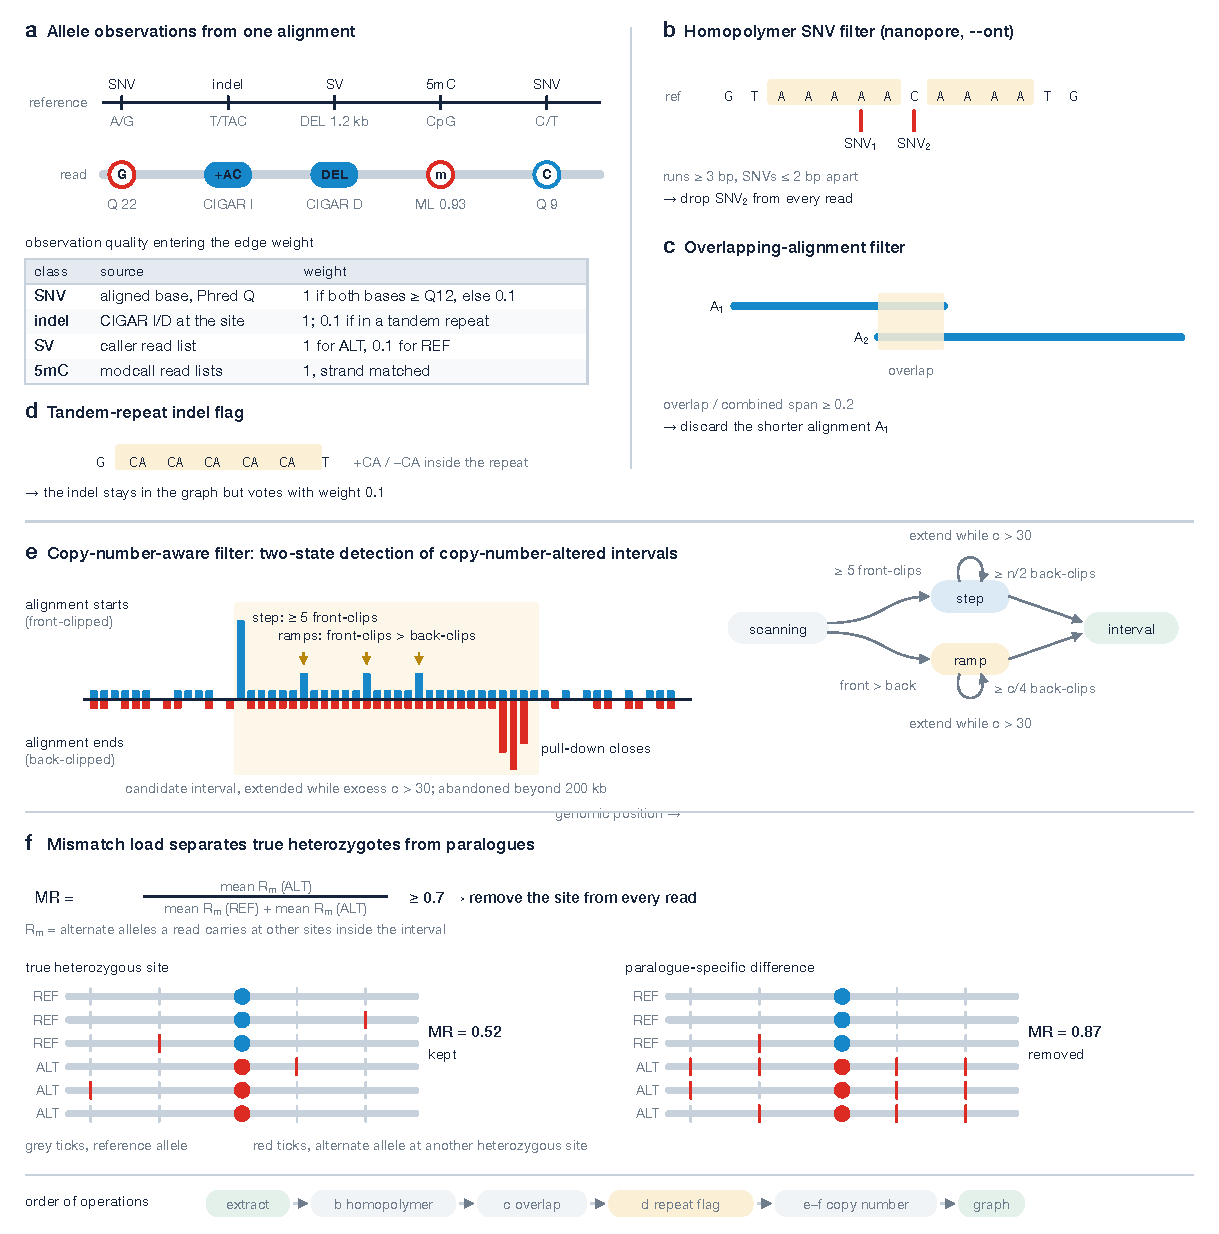
\includegraphics[width=\textwidth]{figures/supp/suppfig1_observations.pdf}
\caption{\textbf{Read-level allele observations and pre-graph filters.}
\textbf{a}, For every alignment, each overlapped variant yields an allele observation with an associated quality: SNVs from the aligned base (Phred quality), indels from CIGAR operations starting at the site, SVs from CIGAR operations of matching length or from the caller's read list, and 5mC from the \code{modcall} read lists. The table summarizes how each class enters the edge weights.
\textbf{b}, Homopolymer SNV filter, applied under \code{--ont}: when two SNVs both lie in homopolymers of length $\ge 3$ and are $\le 2$~bp apart, the downstream SNV is removed.
\textbf{c}, Overlapping-alignment filter for supplementary alignments of one read.
\textbf{d}, Indels in tandem repeats are flagged and vote with weight 0.1.
The strip at the bottom gives the order in which the filters are applied; the copy-number-aware filter of Supplementary Fig.~4 acts last, immediately before graph construction.}
\end{figure}

\begin{figure}[h]
\centering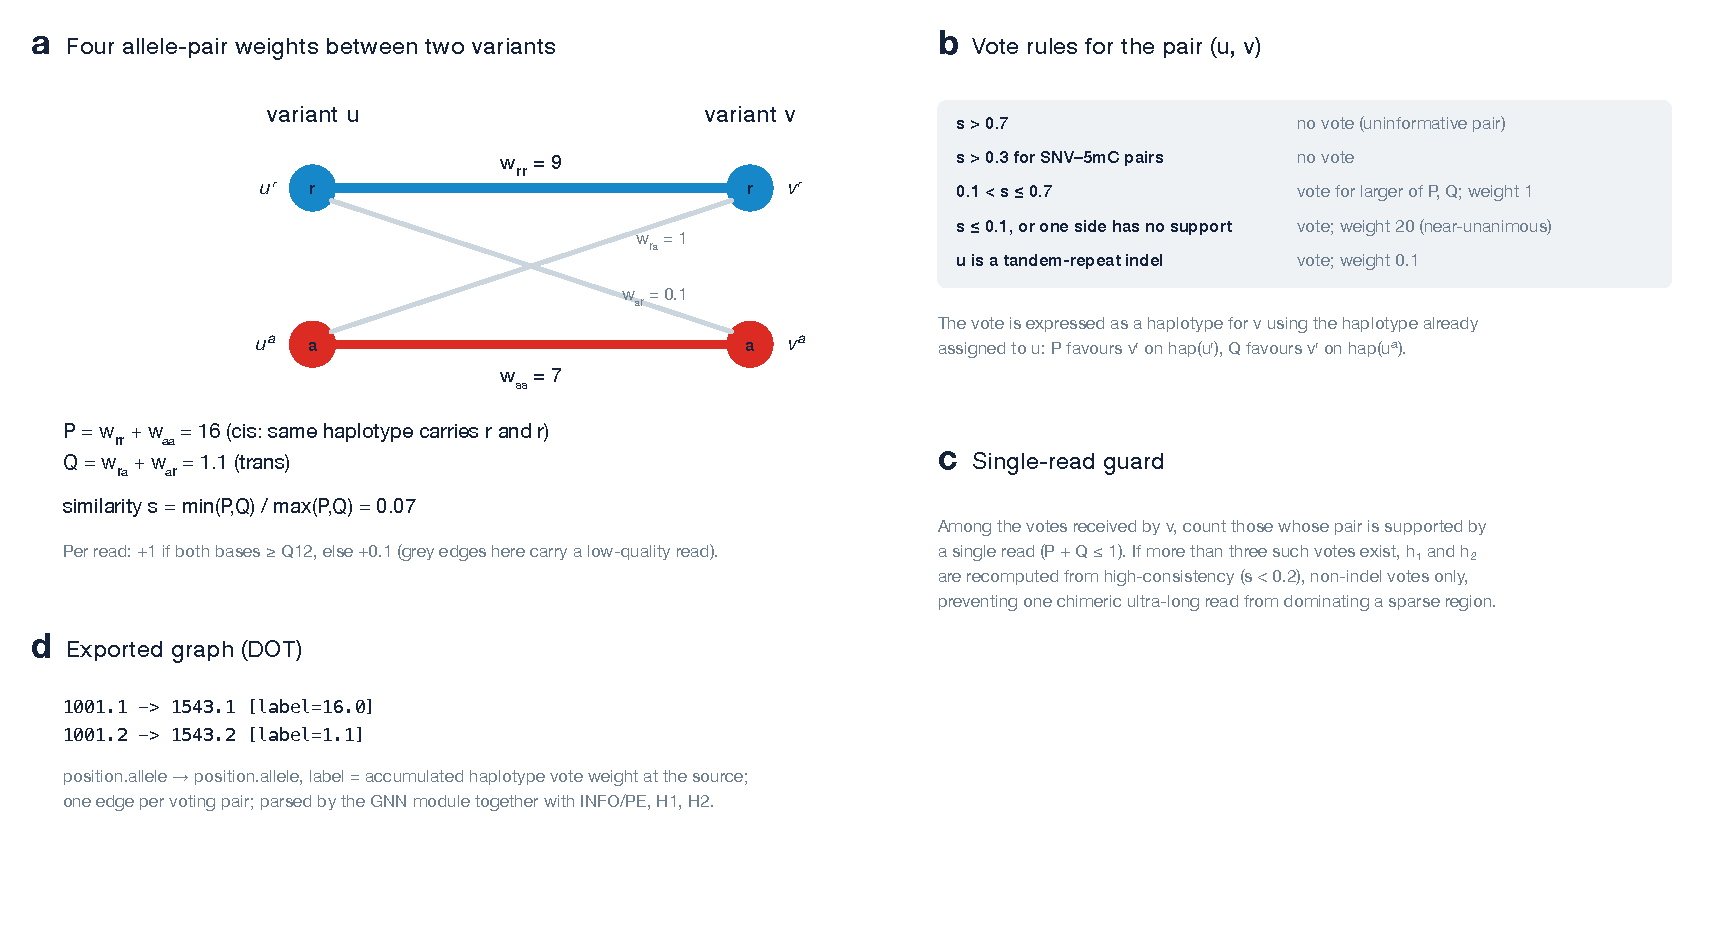
\includegraphics[width=\textwidth]{figures/supp/suppfig2_pair_support.pdf}
\caption{\textbf{Pairwise allele support and vote weighting.}
\textbf{a}, Between two variants $u$ and $v$ the reads accumulate four weights ($w_{rr}, w_{ra}, w_{ar}, w_{aa}$); each read adds 1 when both bases have quality $\ge$~Q12 and 0.1 otherwise. $P$ and $Q$ are the supports for the two possible pairings and $s$ their similarity.
\textbf{b}, Decision rules that turn $(P, Q, s)$ into a weighted haplotype vote for $v$.
\textbf{c}, Guard against a single erroneous ultra-long read: among the votes received by $v$, those whose pair is supported by a single read ($P + Q \le 1$, amber) are counted, and if more than three such votes exist $h_1$ and $h_2$ are recomputed from high-consistency ($s < 0.2$), non-indel votes only.
\textbf{d}, Format of the exported DOT graph consumed by the \code{gnn} module.}
\end{figure}

\begin{figure}[h]
\centering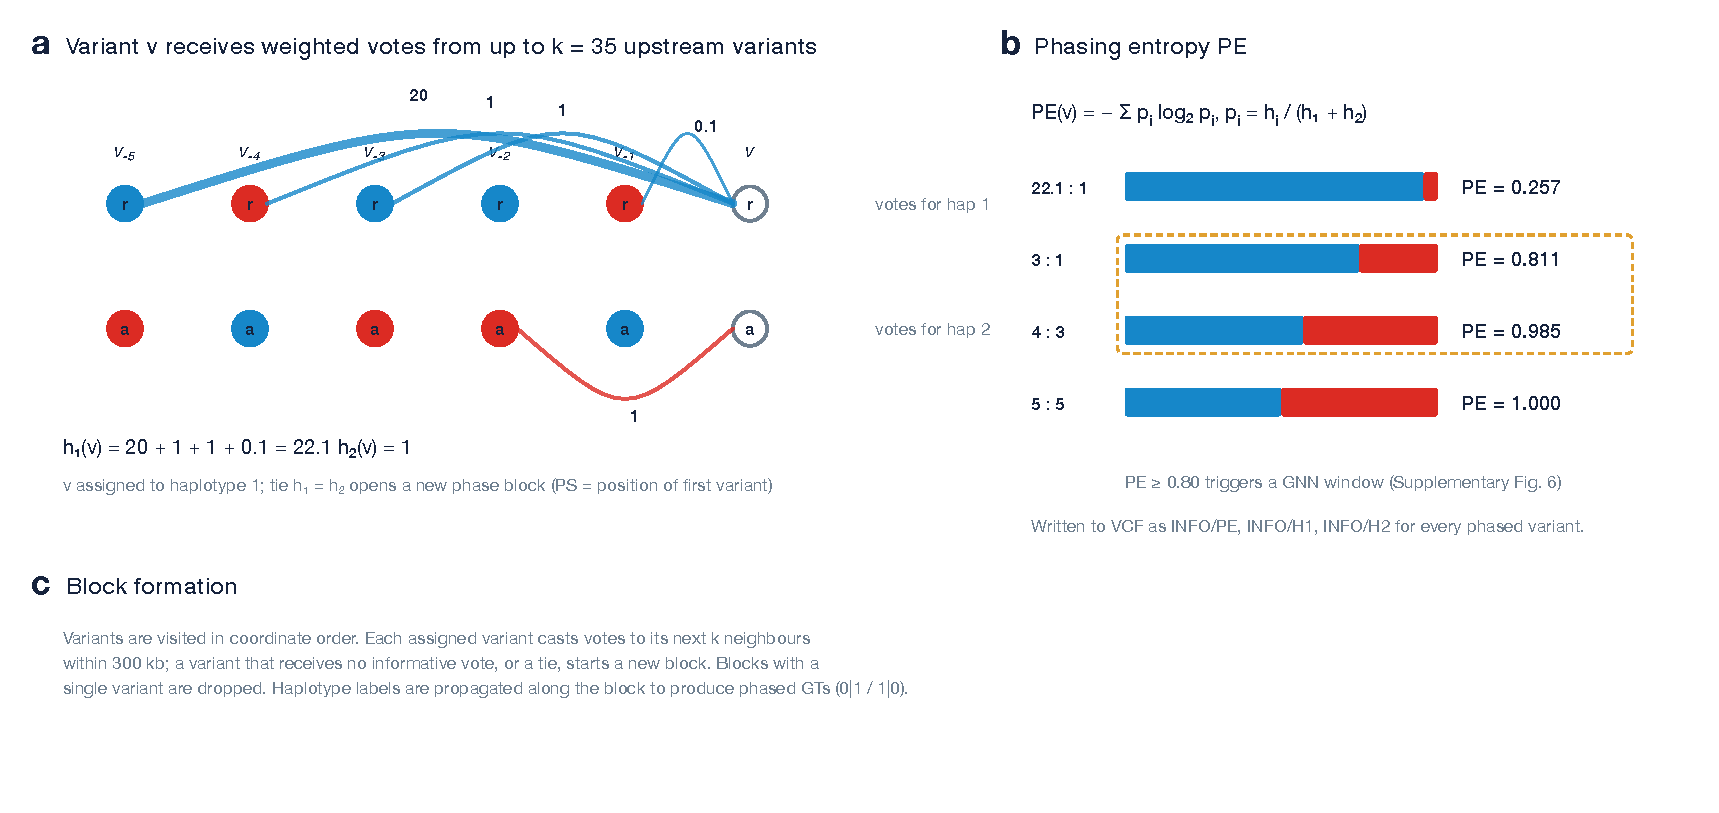
\includegraphics[width=\textwidth]{figures/supp/suppfig3_voting_entropy.pdf}
\caption{\textbf{Multi-neighbour voting and phasing entropy.}
\textbf{a}, Variant $v$ receives weighted votes from up to $k = 35$ upstream variants within 300~kb; line thickness encodes vote weight (20, 1 or 0.1). The haplotype with the larger total wins; a tie opens a new phase block.
\textbf{b}, Phasing entropy of the vote totals for four examples; values $\ge 0.80$ (dashed box) trigger a GNN window.
\textbf{c}, Block formation. Variants are visited in coordinate order and each assigned variant casts votes to its next $k$ neighbours within 300~kb; a variant that receives no informative vote, or a tie, starts a new block (amber). Blocks holding a single variant are dropped (grey). Haplotype labels are propagated along the block to give the phased genotypes 0|1 and 1|0, and the phase set is the position of the first variant of the block.}
\end{figure}

\begin{figure}[h]
\centering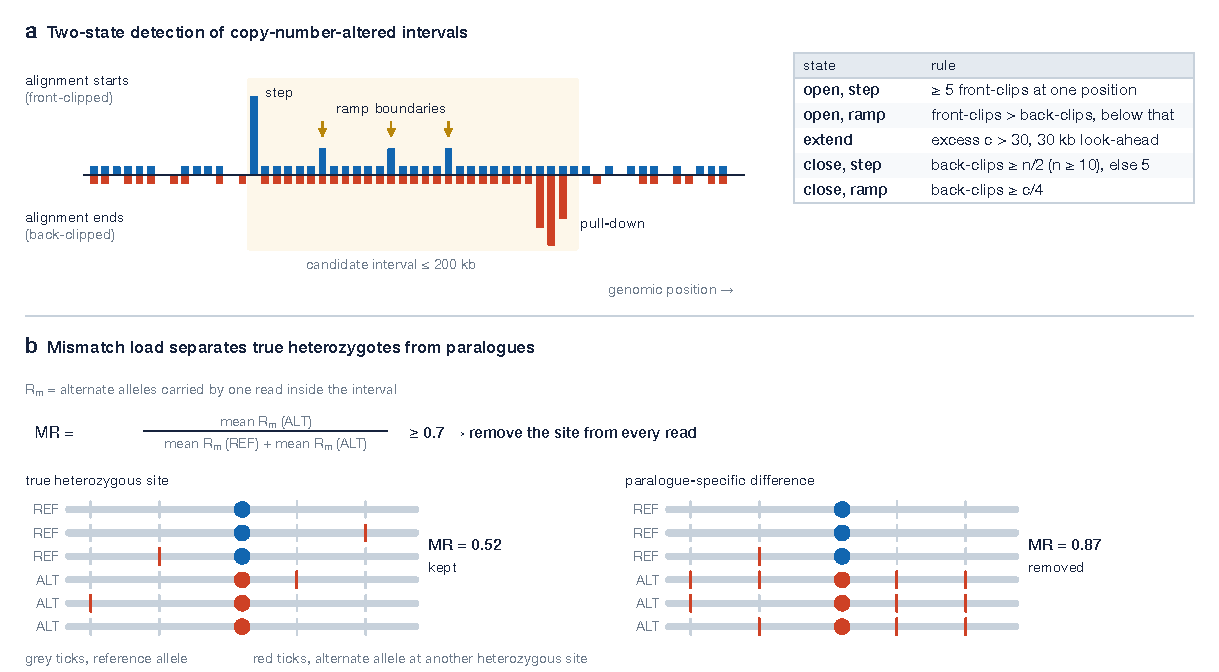
\includegraphics[width=\textwidth]{figures/supp/suppfig4_cnv_filter.pdf}
\caption{\textbf{Copy-number-aware filtering of unreliable heterozygous sites.}
\textbf{a}, Per-position counts of alignments starting (front-clipped, above the axis) and ending (back-clipped, below) are scanned by a two-state detector. A \emph{step} boundary ($\ge 5$ front-clips at one position) marks a copy-number transition; a \emph{ramp} boundary (front-clips exceeding back-clips without reaching that threshold) marks the nested breakpoints left by breakage--fusion--bridge cycles. Both states carry a running excess $c$ of front- over back-clips and extend the candidate end by a 30~kb look-ahead while $c > 30$; a step closes at an adaptive pull-down threshold ($n/2$ for an opening front-clip count $n \ge 10$, else 5) or when $c$ decays to its floor, a ramp closes when back-clips reach $c/4$. Candidates longer than 200~kb are abandoned.
\textbf{b}, Inside an interval, each read is scored by its mismatch load $R_m$ --- the number of heterozygous sites in the interval at which it carries the alternate allele --- and each heterozygous site by $\mathrm{MR} = \bar{R}_m^{\,\mathrm{ALT}}/(\bar{R}_m^{\,\mathrm{REF}}+\bar{R}_m^{\,\mathrm{ALT}})$. At a genuine heterozygous site both allele populations are ordinary reads of the locus and $\mathrm{MR} \approx 0.5$; at a paralogue-specific difference the alternate allele is carried by reads that originate elsewhere and mismatch the reference at many other sites in the same interval, so $\mathrm{MR} \rightarrow 1$. Sites with $\mathrm{MR} \ge 0.7$ are removed from all reads. Sites at which either mean is zero are never removed.
\todo{Add a panel \textbf{c}: the TP/FP histogram of $\mathrm{MR}$ on HG002, with the 0.7 threshold marked. This figure already exists in the group's algorithm slides and shows the separation directly; regenerate it with the submitted version on the Clair3 calls used here, since the slide version predates it. Without it the threshold is asserted rather than shown.}}
\end{figure}

\begin{figure}[h]
\centering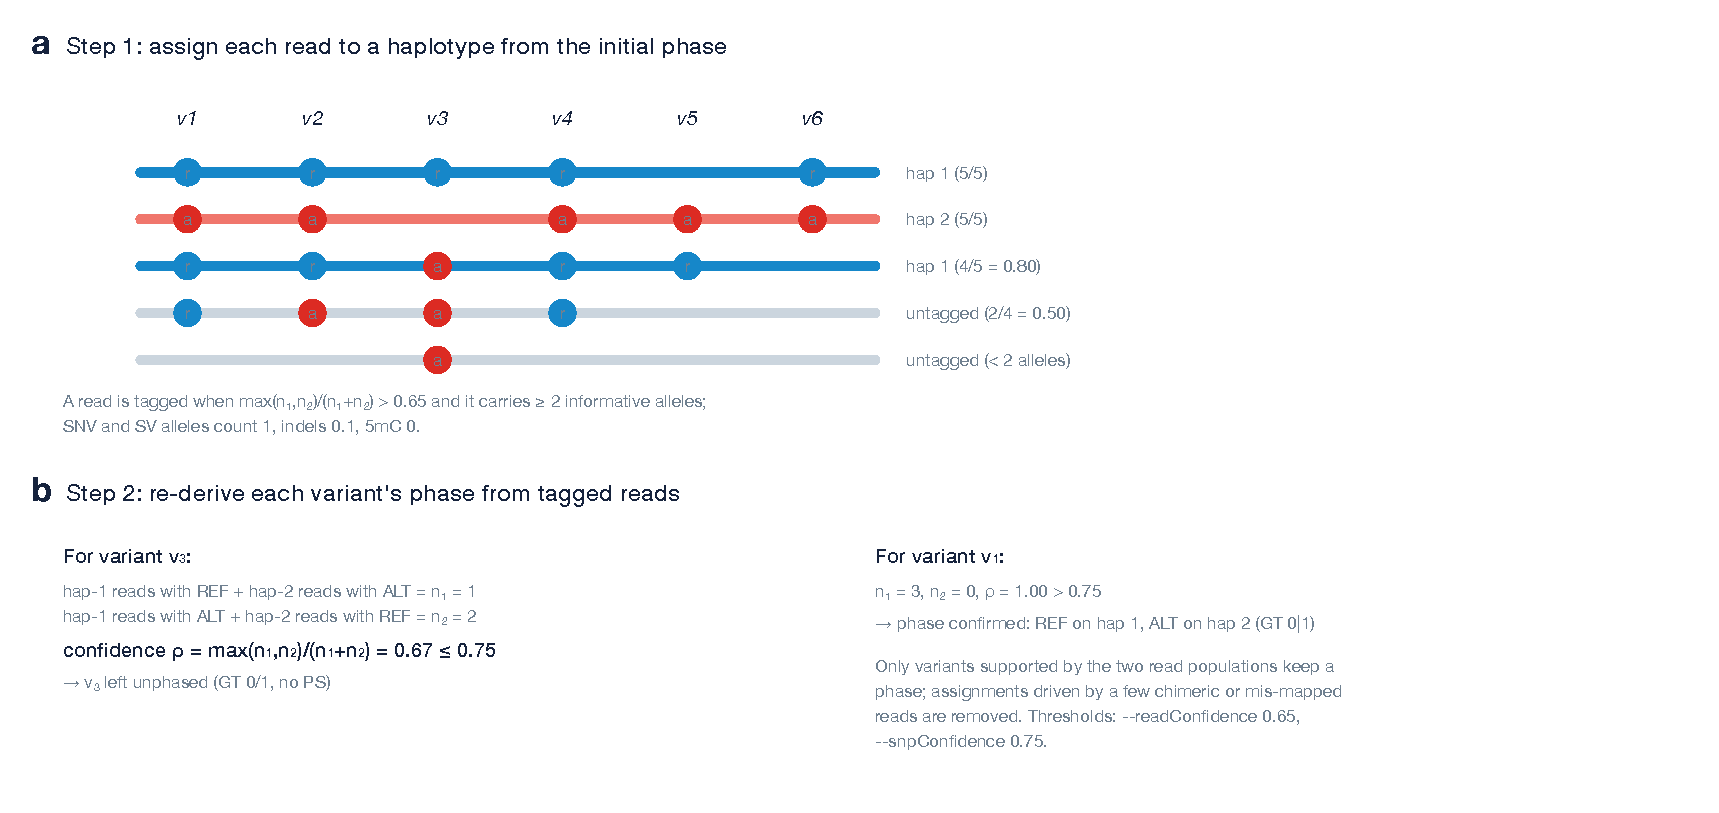
\includegraphics[width=\textwidth]{figures/supp/suppfig5_read_correction.pdf}
\caption{\textbf{Read-based correction.}
\textbf{a}, Each read is assigned to a haplotype by majority over its phased SNV and SV alleles (indels count 0.1, 5mC 0); reads with majority $\le 0.65$ or fewer than two informative alleles remain untagged.
\textbf{b}, Each variant's phase is re-derived from the tagged reads and retained only if the consistent fraction $\rho$ exceeds 0.75; otherwise the variant is unphased. Only variants supported by both read populations keep a phase, so assignments driven by a few chimeric or mis-mapped reads are removed. The two thresholds are \code{--readConfidence} 0.65 and \code{--snpConfidence} 0.75.}
\end{figure}

\begin{figure}[h]
\centering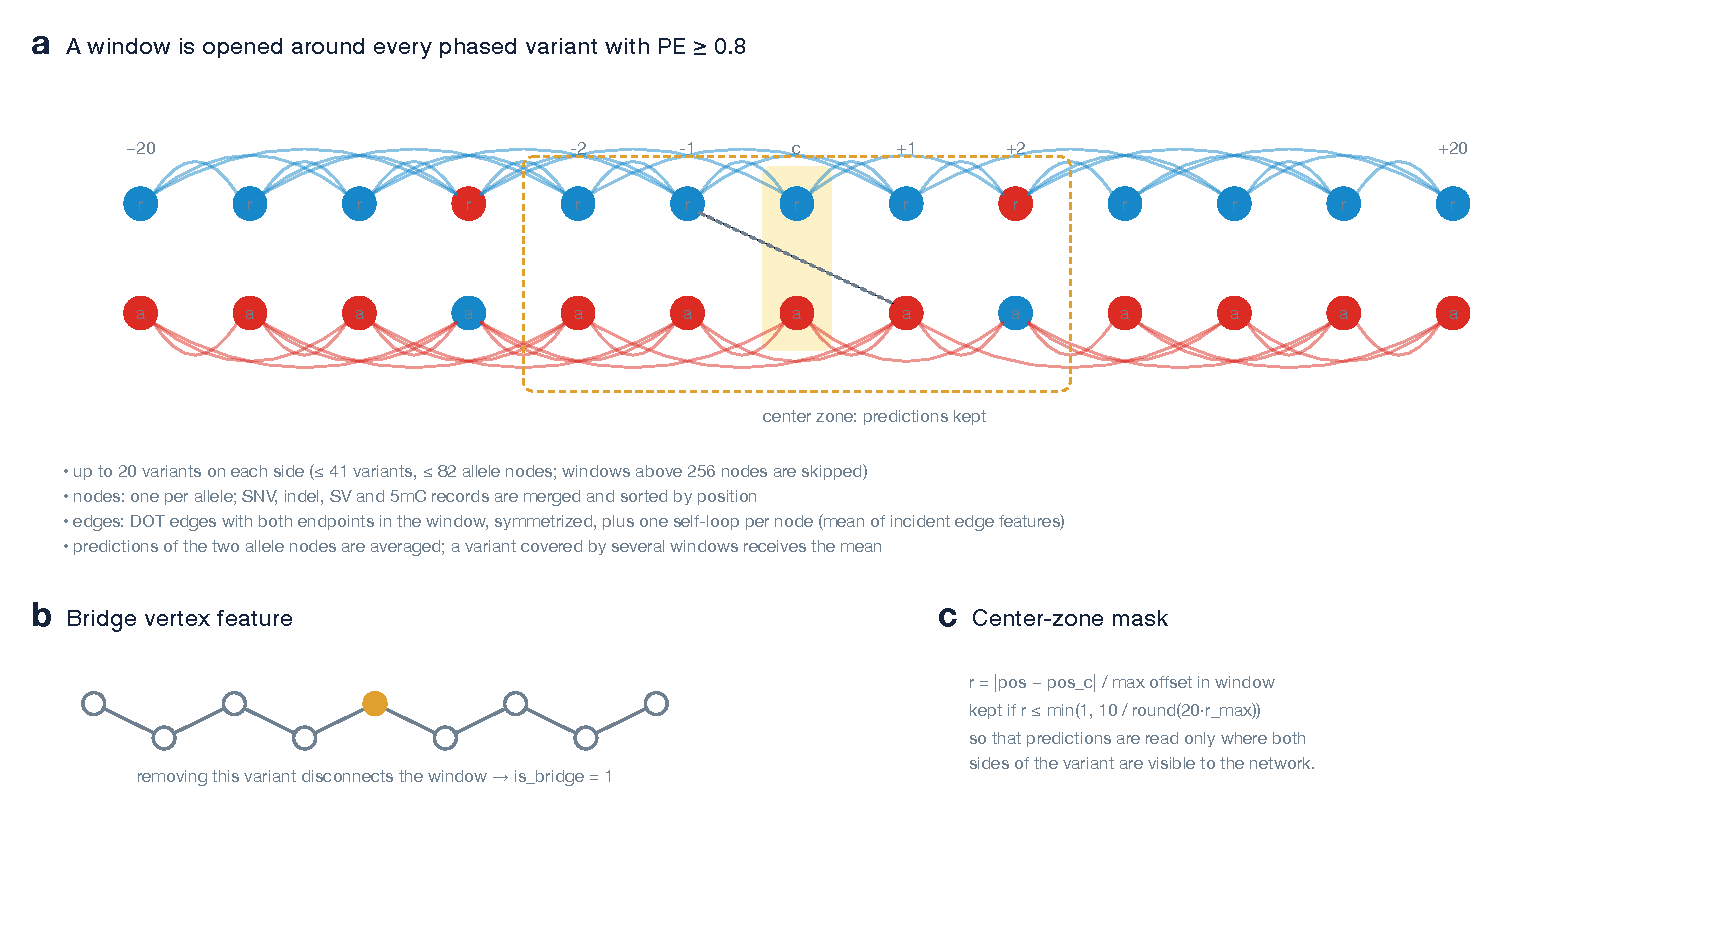
\includegraphics[width=\textwidth]{figures/supp/suppfig6_gnn_window.pdf}
\caption{\textbf{Window construction for the graph neural network.}
\textbf{a}, A window of $\pm 20$ variants (two allele nodes each) is opened around every phased variant with PE $\ge 0.8$; edges are the DOT edges with both endpoints in the window (blue and red arcs) plus self-loops; a dashed grey edge marks a cross-haplotype link. Predictions are read only in the central zone.
\textbf{b}, Bridge-vertex feature: a variant whose removal disconnects the window graph.
\textbf{c}, Definition of the central zone. A window holds at most 41 variants and 82 allele nodes (a 256-node cap exists but is never reached at the default window size); SNV, indel, SV and 5mC records are merged and sorted by position before nodes are created. Because offsets are normalized by the largest offset in the window, $r_{\max}=1$ in practice and the retained zone is the central half of the window's genomic span. Edges are the DOT edges with both endpoints in the window, symmetrized, plus one self-loop per node whose features are the mean over that node's incident edges. The predictions of the two allele nodes of a variant are averaged, and a variant covered by several windows receives the mean over those windows.}
\end{figure}

\begin{figure}[h]
\centering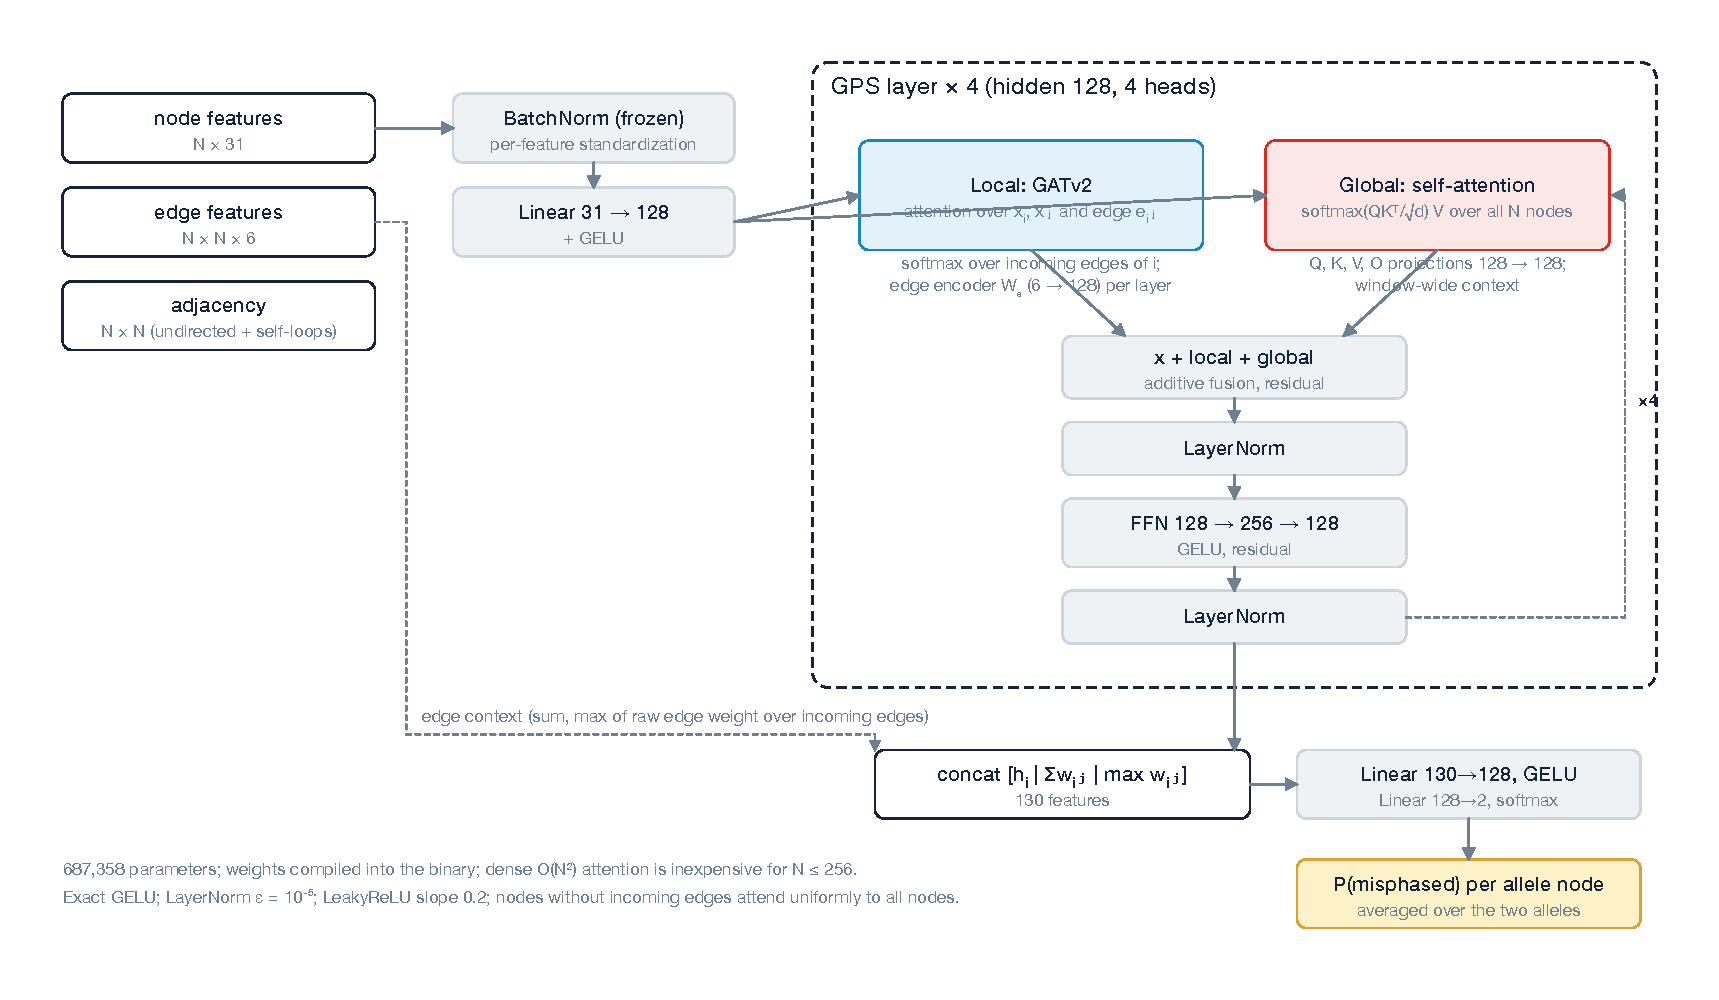
\includegraphics[width=\textwidth]{figures/supp/suppfig7_gnn_architecture.pdf}
\caption{\textbf{Graph neural network architecture.} Node features are standardized and projected to 128 dimensions. Each of four GPS layers combines a local GATv2 branch over the window graph (edge features enter through a per-layer edge encoder) with a global self-attention branch over all nodes, fused additively into the residual stream and followed by layer normalization and a feed-forward block. The final embedding is concatenated with the sum and maximum of incoming raw edge weights and classified into phased-correctly versus misphased; the probabilities of the two allele nodes of a variant are averaged.}
\end{figure}

\begin{figure}[h]
\centering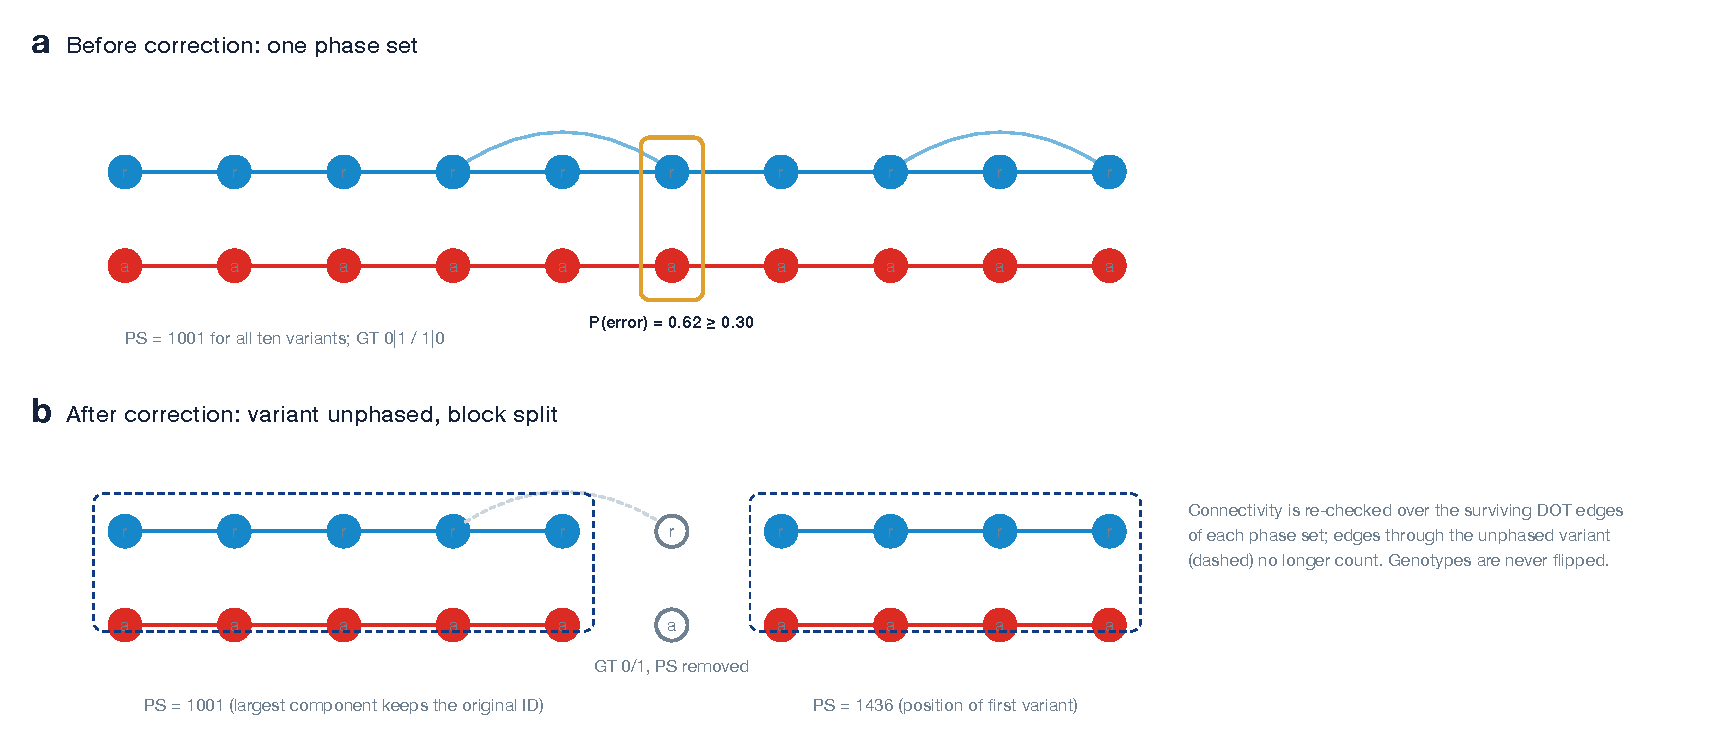
\includegraphics[width=\textwidth]{figures/supp/suppfig8_unphase_split.pdf}
\caption{\textbf{Unphasing and phase-set splitting.}
\textbf{a}, A variant with predicted error probability $\ge 0.30$ (amber) inside a phase set.
\textbf{b}, After correction the variant is written as an unphased genotype without PS; connectivity of the remaining variants is recomputed over the surviving DOT edges, the largest component keeps the original PS and every other component receives a new PS equal to the position of its first variant. Genotypes are never flipped.}
\end{figure}

\begin{figure}[h]
\centering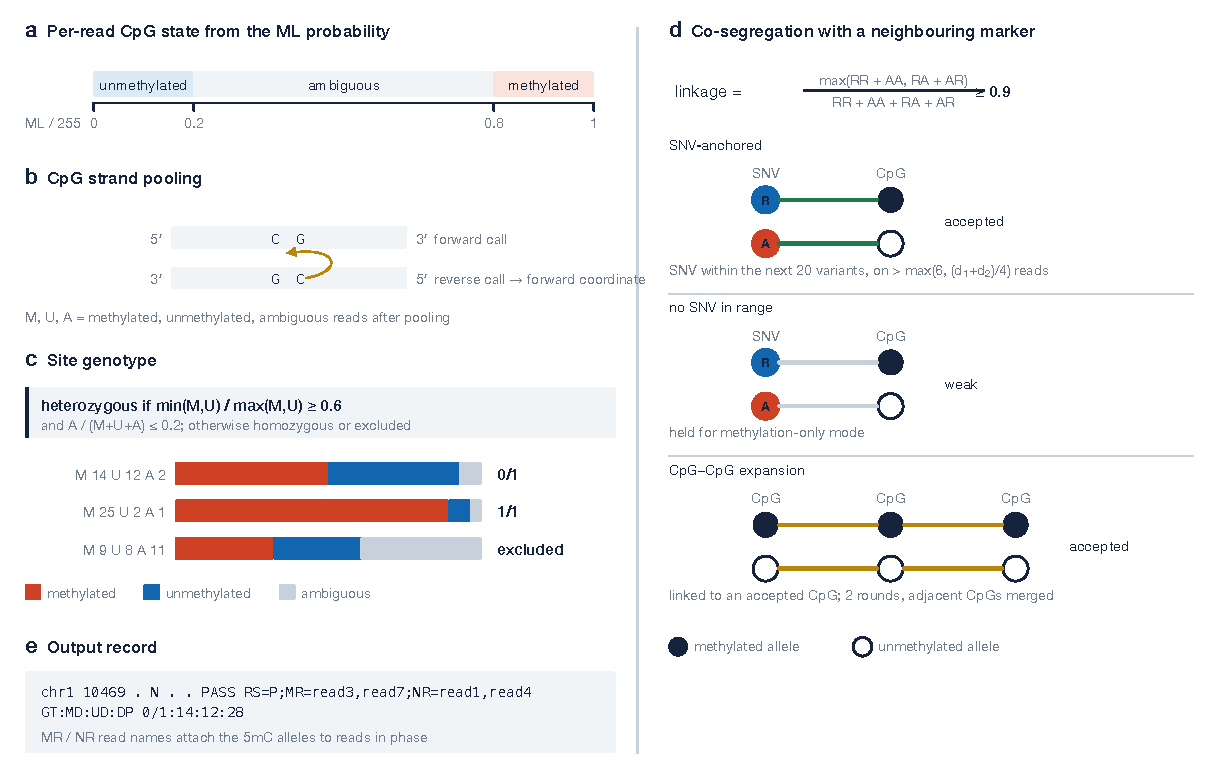
\includegraphics[width=\textwidth]{figures/supp/suppfig9_modcall.pdf}
\caption{\textbf{Allele-specific methylation calling with \code{modcall}.}
\textbf{a}, Per-read CpG state is read from the \code{MM}/\code{ML} tags on both strands: methylated at \code{ML}/255 $\ge 0.8$, unmethylated at $\le 0.2$, ambiguous in between. Only CpG dinucleotides are considered.
\textbf{b}, 5mC is called on one strand at a time, so reverse-strand calls are mapped to the forward CpG coordinate and runs of consecutive CpGs are merged into a single locus carrying one read list. This removes strand from the problem and lets \code{phase} vote on methylation loci with the unmodified graph algorithm.
\textbf{c}, A site is heterozygous when $\min(M,U)/\max(M,U) \ge 0.6$ and $A/(M+U+A) \le 0.2$, for methylated, unmethylated and ambiguous read counts $M$, $U$ and $A$; otherwise it is homozygous and excluded.
\textbf{d}, Balance alone does not imply allele specificity, since stochastic methylation satisfies \textbf{c} as well. Read support between two loci is therefore decomposed into the four state pairs, whose concordant and discordant totals are exactly the quantities $P$ and $Q$ that the phasing graph accumulates (\code{VariantEdge::findNumberOfRead}); a pair is linked when $\max(P,Q)/(P+Q) \ge 0.9$. The example shown falls below the threshold and is rejected.
\textbf{e}, Linking runs in three modes: against an SNV among the next 20 variants, against another candidate CpG where no informative SNV is in range, and an iterative expansion that admits weak candidates against an already accepted CpG. In every mode a pair is considered only while the reads spanning it exceed $\max(6,(n_1+n_2)/4)$, and falling to that bound ends the neighbour scan for that site rather than skipping one pair.
\textbf{f}, Output record; the \code{MR} and \code{NR} read names attach the 5mC alleles to reads in \code{phase}.
\todo{Two real-data panels would close the remaining gaps, and both exist in the group's thesis material. (i)~Per-site \code{ML} probability at heterozygous versus homozygous CpGs with the 0.8 and 0.2 lines marked, showing that it is the homozygous sites that spread across the ambiguous band; the original was computed on 48 sites in the imprinted \textit{SNRPN} locus, too small and too special a sample for a Nature Methods supplement, so recompute genome-wide on HG002. (ii)~Distribution of the linkage ratio in \textbf{d} stratified by the true class of the site pair (heterozygous--heterozygous, homozygous--homozygous, heterozygous--homozygous). This is the strongest justification available for the 0.9 threshold: in the original the three classes separate at roughly 0.65--1, 0.5--0.75 and 0.5--0.7, showing that the cut removes homozygous sites misclassified as allele-specific rather than being an arbitrary round number. Regenerate both with the submitted version.}}
\end{figure}

\begin{figure}[h]
\centering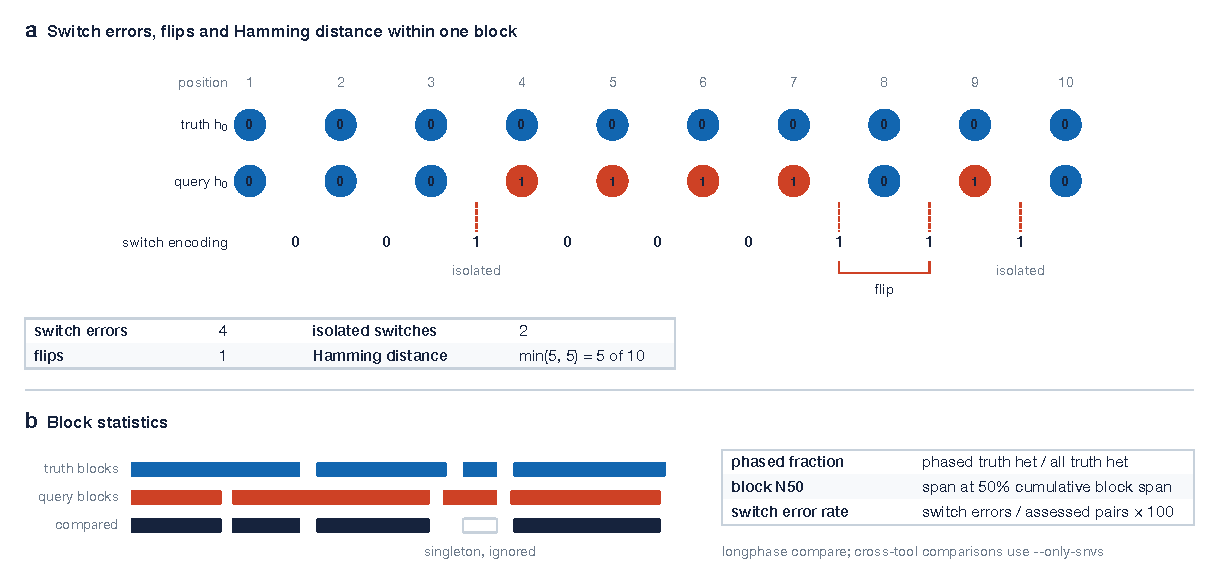
\includegraphics[width=\textwidth]{figures/supp/suppfig10_metrics.pdf}
\caption{\textbf{Phasing evaluation metrics.}
\textbf{a}, Within one intersected block, the query haplotype string is compared with the truth in switch encoding; the number of differing positions is the switch-error count, adjacent switch pairs are counted as flips, and the Hamming distance is the minimum over the two orientations of misassigned variants.
\textbf{b}, Block intersection and the block-level statistics. Only variants that are heterozygous in both files and phased in both are compared (dark bars); blocks left with a single variant are ignored (outline). Phased fraction, block N50 and switch error rate are computed over the intersected blocks as implemented in \code{longphase compare}.}
\end{figure}

\begin{figure}[h]
\centering
\fbox{\begin{minipage}{0.97\textwidth}\vspace{3em}\centering\small\itshape Placeholder --- panels to be regenerated with the submitted version.\vspace{3em}\end{minipage}}
\caption{\textbf{Calibration of the voting and read-filtering constants.} Each panel is a sweep on HG002 at 10--60$\times$; the value adopted in \toolname is marked.
\textbf{a}, Distribution of pair ambiguity $s=\min(P,Q)/\max(P,Q)$ over all assessed pairs and over the subset that participate in a switch error, showing that both mass and residual error concentrate below $s=0.1$ and motivating $\alpha = 0.1$ as the boundary of the up-weighted class.
\textbf{b}, Switch errors and block N50 as a function of the no-vote threshold $\beta$. Switch errors fall monotonically as $\beta$ decreases, so switch error alone does not identify an optimum; $\beta = 0.7$ is the smallest value at which block N50 is not yet degraded, and is adopted on that basis.
\textbf{c}, Switch errors as a function of the up-weight $w$ applied when $s < \alpha$, at each coverage; the reduction saturates by $w \approx 20$.
\textbf{d}, Distribution of base quality over all bases and over bases carrying a sequencing error, showing errors concentrated below Q10 and motivating $\theta = 12$; and switch errors as a function of $\theta$.
\textbf{e}, Switch errors over the grid of single-read-guard parameters $N$ (number of single-read votes that triggers the guard) and $\mu$ (ambiguity cut applied to the surviving votes), and switch errors with and without the guard at each coverage.
\todo{All five panels exist as figures in the group's thesis material (Po-Hui Tzeng, 2026, Figs.~3.7, 3.10--3.12, 3.14, 3.17, 3.18, 3.21) and should be regenerated with the submitted version on the Clair3 calls and coverages used here, then redrawn to a single consistent style. Two caveats to carry over honestly: in \textbf{b} the switch-error curve does not have an interior optimum, so the choice of $\beta$ rests on the N50 trade-off and must be presented that way; and in \textbf{e} the guard slightly \emph{increased} switch errors at 10$\times$ in the original sweep, which should be shown rather than cropped.}}
\label{fig:supp_calibration}
\end{figure}

\clearpage
\bibliography{references}
\end{document}
